% MICCAI 2027 draft v0 (2026-10-26). Pathology only; the
% natural-image half of the CVPR draft (../cvpr) is out of scope here. Numbers: tab_main.tex <- ../../analysis/miccai_table.py;
% redundancy CIs: ../../results/ext/SUMMARY_red.md. Red \pend{} = result running (Killarney arch jobs) or to verify.
\documentclass[runningheads]{llncs}
\usepackage{graphicx,booktabs,amsmath,amssymb,multirow,xcolor,tikz}
\usetikzlibrary{arrows.meta}
\usepackage[colorlinks,allcolors=blue]{hyperref}
\newcommand{\pend}[1]{{\color{red}[#1]}}
\newcommand{\authnote}[1]{{\color{blue}[Note: #1]}}
\newcommand{\pmsd}[1]{{\tiny$\pm$#1}}
\begin{document}
\title{Whoever Picks the Tiles Decides: Selection Attacks on Efficient Whole-Slide Classifiers}
\titlerunning{Selection Attacks on Efficient Whole-Slide Classifiers}
\author{Anonymized Authors}\authorrunning{Anonymized Author et al.}\institute{Anonymized Affiliations\\\email{email@anonymized.com}}
\maketitle

\begin{abstract}
Efficient whole-slide image (WSI) classifiers let a cheap model pick a few tiles and encode only those with a pathology foundation model. We show that this tile selector is a single point of failure. An attacker who controls only the selector, and shows nothing but real, unmodified tiles from the slide, decides the diagnosis. On CAMELYON17, TCGA-RCC and TCGA-NSCLC, a compromised selector sends an ADMIL-style pipeline to the attacker's class on nearly every slide ($\kappa=-.24$; balanced accuracy .02 and .00). Neither a larger tile budget nor \pend{a different MIL aggregator} prevents this, while an honest but weak selector costs at most .01. The fragility is therefore adversarial, not statistical. We then ask how to present tiles so that no single selection component decides. One advocate per diagnosis, as in debate, fails exactly where it matters: if the attacker takes the true class's advocate, the judge sees evidence only for wrong classes (.59/.43/.15). Plain redundancy, i.e.\ several slots that each show the selector's top tiles, restores the worst case to .65--.75 at the cost of a few more encoded tiles, with clean accuracy within .01 of the single selector. Which form of redundancy is best (one judge over all slots, or each slot judged alone) depends on the cohort.
\keywords{Multiple-instance learning \and Adversarial robustness \and Efficient WSI inference}
\end{abstract}

%=====================================================================
\section{Introduction}
\authnote{opening: one concrete clinical scene. A slide-level classifier that only reads the tiles a triage model hands it; the triage model is third-party, outsourced, swapped in an update, or buggy. Whoever controls that hand-off controls the diagnosis, and every tile the pathologist would check is real.}

A gigapixel WSI holds thousands of tiles, and encoding all of them with a pathology foundation model~\cite{uni,conch} is the main cost of slide-level inference. Efficient pipelines therefore \emph{select}: a cheap low-magnification model scores every tile, and only the top few are encoded and aggregated by a multiple-instance learning (MIL) model~\cite{thandiackal2022zoommil,zhao2023rlogist,admil2026,eagle2026}. With 8--16 tiles out of 2,000--4,300 (0.2--0.8\%), such a pipeline is within .014--.026 of full-slide MIL in our experiments.

We study what happens when the selector cannot be trusted. Our attacker is deliberately weak in what it may \emph{show}: it never perturbs a pixel or a feature, and it shows no more tiles than the honest selector. It only chooses \emph{which} real tiles of the slide are presented. Attacks on MIL usually perturb tile pixels or features~\cite{foote2021now,mil_adv2022}, and defences against them do not apply here, because every presented tile is genuine and would pass a pathologist's review one at a time.

\textbf{Contributions.} (1) A threat model for tile selection in efficient WSI classifiers, with a per-tile and a judge-aware adaptive attacker. (2) Evidence that the single selector collapses under this attack on three cohorts, at 1--2$\times$ the tile budget and \pend{for four MIL aggregators}, while honest weak selectors cost $\le$.01. (3) The finding that per-class advocates fail when the true class's advocate is compromised, even with independently trained scorers. (4) An evaluation of redundant presenters (3 seeds $\times$ 5 folds, paired CIs), showing that plain redundancy restores most of the worst case and that the best variant depends on the cohort.

%=====================================================================
\section{Related Work}
\textbf{Efficient WSI inference.} MIL on foundation-model features~\cite{ilse2018abmil,lu2021data,shao2021transmil,li2021dual} reads every tile. ZoomMIL~\cite{thandiackal2022zoommil}, RLogist~\cite{zhao2023rlogist}, ADMIL~\cite{admil2026} and EAGLE~\cite{eagle2026} select a few tiles with a cheap model first. Recent work measures how selection shifts the evidence MIL sees~\cite{bagshift2026,foci2026} and regularises attention to be faithful~\cite{gcemil2026,carmil2026}. None considers a compromised selector.
\textbf{Adversarial attacks on pathology.} Attacks on MIL perturb pixels or features~\cite{foote2021now,mil_adv2022}. Our attacker does neither.
\textbf{Debate and redundancy.} Debate~\cite{irving2018debate,khan2024debate}, prover--verifier games~\cite{anil2021pvg} and Merlin--Arthur classifiers~\cite{waldchen2024merlin} let untrusted provers present evidence to a verifier; our advocates follow this idea. Isolate-then-aggregate defences judge each retrieved passage or image region separately and aggregate~\cite{xiang2024robustrag,xiang2022patchcleanser}; our isolated redundancy is the WSI analogue.

\begin{figure}[t]\centering
\resizebox{\textwidth}{!}{% Method figure (MICCAI): four presenters, each with one compromised slot (red). \input inside a figure (needs tikz, arrows.meta).
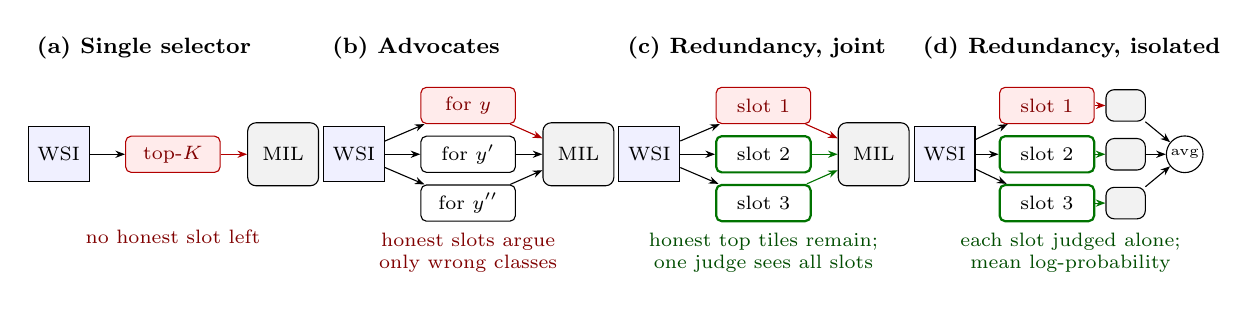
\begin{tikzpicture}[font=\scriptsize, >={Stealth[length=3.5pt]},
  slot/.style={draw, rounded corners=2pt, minimum width=12mm, minimum height=4.6mm, align=center, fill=white, inner sep=1pt},
  bad/.style={slot, draw=red!70!black, fill=red!8, text=red!50!black},
  wit/.style={slot, draw=green!45!black, line width=.8pt},
  judge/.style={draw, rounded corners=3pt, minimum width=9mm, minimum height=8mm, align=center, fill=gray!10},
  img/.style={draw, minimum width=7mm, minimum height=7mm, fill=blue!6},
  ttl/.style={font=\footnotesize\bfseries, anchor=west}]
\begin{scope}
  \node[ttl] at (-0.4, 1.35) {(a) Single selector};
  \node[img] (x) at (0, 0) {WSI}; \node[bad] (s) at (1.45, 0) {top-$K$};
  \node[judge] (j) at (2.85, 0) {MIL}; \draw[->] (x) -- (s); \draw[->, red!70!black] (s) -- (j);
  \node[align=center, text=red!50!black] at (1.45, -1.05) {no honest slot left};
\end{scope}
\begin{scope}[xshift=3.75cm]
  \node[ttl] at (-0.4, 1.35) {(b) Advocates};
  \node[img] (x) at (0, 0) {WSI};
  \node[bad] (a1) at (1.45, 0.62) {for $y$}; \node[slot] (a2) at (1.45, 0) {for $y'$}; \node[slot] (a3) at (1.45, -0.62) {for $y''$};
  \node[judge] (j) at (2.85, 0) {MIL};
  \foreach \s in {a1,a2,a3} \draw[->] (x) -- (\s); \draw[->, red!70!black] (a1) -- (j); \draw[->] (a2) -- (j); \draw[->] (a3) -- (j);
  \node[align=center, text=red!50!black] at (1.45, -1.25) {honest slots argue\\only wrong classes};
\end{scope}
\begin{scope}[xshift=7.5cm]
  \node[ttl] at (-0.4, 1.35) {(c) Redundancy, joint};
  \node[img] (x) at (0, 0) {WSI};
  \node[bad] (r1) at (1.45, 0.62) {slot 1}; \node[wit] (r2) at (1.45, 0) {slot 2}; \node[wit] (r3) at (1.45, -0.62) {slot 3};
  \node[judge] (j) at (2.85, 0) {MIL};
  \foreach \s in {r1,r2,r3} \draw[->] (x) -- (\s); \draw[->, red!70!black] (r1) -- (j);
  \draw[->, green!45!black] (r2) -- (j); \draw[->, green!45!black] (r3) -- (j);
  \node[align=center, text=green!30!black] at (1.45, -1.25) {honest top tiles remain;\\one judge sees all slots};
\end{scope}
\begin{scope}[xshift=11.25cm]
  \node[ttl] at (-0.4, 1.35) {(d) Redundancy, isolated};
  \node[img] (x) at (0, 0) {WSI};
  \node[bad] (r1) at (1.3, 0.62) {slot 1}; \node[wit] (r2) at (1.3, 0) {slot 2}; \node[wit] (r3) at (1.3, -0.62) {slot 3};
  \foreach \s/\yy in {r1/0.62,r2/0,r3/-0.62} { \draw[->] (x) -- (\s); \node[judge, minimum width=5mm, minimum height=4mm] (j\s) at (2.3, \yy) {}; }
  \draw[->, red!70!black] (r1) -- (jr1); \draw[->, green!45!black] (r2) -- (jr2); \draw[->, green!45!black] (r3) -- (jr3);
  \node[draw, circle, inner sep=1pt] (m) at (3.05, 0) {\tiny avg}; \foreach \s in {r1,r2,r3} \draw[->] (j\s) -- (m);
  \node[align=center, text=green!30!black] at (1.6, -1.25) {each slot judged alone;\\mean log-probability};
\end{scope}
\end{tikzpicture}
}
\caption{\textbf{Presenters under one compromised slot} (red). (a) A compromised single selector decides alone. (b) With one advocate per class, compromising the true class's advocate leaves only slots that argue for wrong classes. (c, d) With redundant slots that each show the selector's top tiles, honest top tiles remain (green), judged jointly (c) or slot by slot (d).}\label{fig:method}
\end{figure}

%=====================================================================
\section{Method}
\textbf{Setting.} A slide $x$ has tiles $\{t_1,\dots,t_N\}$. A \emph{presenter} has slots $s=1..m$; slot $s$ shows a set $S_s$ of at most $B_s$ tiles, tagged with a one-hot slot flag. The judge $J$, a gated-attention MIL model~\cite{ilse2018abmil} over the foundation-model features of the shown tiles, outputs the class.

\textbf{Threat model.} The attacker compromises \emph{one} slot of its choice and replaces $S_s$ with any $B_s$ tiles of the same slide. It cannot change the other slots, the flags or the features. It knows the true label $y$ and has white-box access to $J$. \emph{Per-tile attack}: for each wrong class $c$, show the $B_s$ tiles with the highest single-tile $\log p_J(c)$ under slot $s$'s flag. \emph{Adaptive attack}: build $S_s$ greedily from the top-128 per-tile candidates, each step adding the tile that minimises $p_J(y)$ given the honest slots. The worst case is taken per slide over slots, target classes and both attacks.

\textbf{Presenters.} \emph{Single selector} (ADMIL-style~\cite{admil2026}): one slot with the top-$K$ tiles by attention of a cheap scorer, an MLP on ImageNet EfficientNet-B0~\cite{tan2019efficientnet} features distilled from a full-slide CONCH~\cite{conch} ABMIL; $K=C K_c$, $K_c=4$. \emph{Advocates}: one slot per class $c$, showing the $K_c$ tiles with the largest cheap-scorer margin for $c$ (stage-specific spatial rules on CAMELYON17, supplement). \emph{Redundancy}: $C{+}1$ unlabelled slots that share the single selector's top $(C{+}1)K_c$ tiles round-robin; any slot may be compromised. It is judged \emph{jointly} (one judge over all slots) or \emph{isolated} (each slot judged alone, mean of per-slot log-probabilities, as in~\cite{xiang2024robustrag}). \emph{Advocates + neutral}: the advocates plus one unlabelled slot with the selector's top $K_c$ or $K$ tiles.

\textbf{Judge training.} The judges of multi-slot presenters are trained on honest presentations and on presentations with one slot replaced by the per-tile attacker, for three rounds, over every (slot, target class) pair the attacker may use. The single selector's judge is the full-slide model.

\textbf{When does redundancy help?} If the attacker compromises one slot, a presenter keeps an honest slot whose tiles support $y$ (a \emph{witness}) unless all such slots were the one compromised. The single selector has one slot and no remaining witness. Advocates have one witness, the advocate of $y$, which the attacker can take. Redundancy and advocates + neutral keep at least one witness under any single compromise. Whether the judge \emph{follows} the remaining witness is an empirical property of the judge, which our worst-case numbers measure. \authnote{tighten into a short proposition for the final version; keep it modest}

%=====================================================================
\section{Experiments}
\textbf{Data.} CAMELYON17~\cite{camelyon17} (500 lymph-node slides, 4 pN stages, leave-one-hospital-out, quadratic-weighted $\kappa$), TCGA-RCC (882 slides, 3 subtypes) and TCGA-NSCLC (1,041 slides, 2 subtypes)~\cite{tcga} (5-fold patient-level CV, balanced accuracy). Tiles at 20$\times$ (CONCH) and at low magnification (EfficientNet-B0). We report the mean over 5 folds, then mean $\pm$ sd over 3 seeds; paired 95\% bootstrap CIs over the 15 fold-seed runs.

\begin{table}[t]\centering
\caption{\textbf{One compromised slot.} $\kappa$ (CAMELYON17) or balanced accuracy (TCGA), clean and worst case over which slot the attacker takes (adaptive attack; per-tile for the single selector, which already reaches the attacker's class, and for independent scorers). Mean\pmsd{sd} over 3 seeds. Full-slide CONCH MIL: .890 / .933 / .923.}\label{tab:main}
\setlength{\tabcolsep}{2pt}\scriptsize
\begin{tabular}{@{}lcccccc@{}}\toprule
 & \multicolumn{2}{c}{CAMELYON17} & \multicolumn{2}{c}{TCGA-RCC} & \multicolumn{2}{c}{TCGA-NSCLC}\\\cmidrule(lr){2-3}\cmidrule(lr){4-5}\cmidrule(lr){6-7}
presenter & clean & worst & clean & worst & clean & worst\\\midrule
single selector & .873\pmsd{.021} & $-$.241\pmsd{.009} & .907\pmsd{.019} & .022\pmsd{.002} & .909\pmsd{.007} & .003\pmsd{.000}\\
\quad budget $K{+}K_c$ & .883\pmsd{.013} & $-$.233\pmsd{.008} & .908\pmsd{.018} & .028\pmsd{.001} & .911\pmsd{.008} & .006\pmsd{.002}\\
\quad budget $2K$ & .891\pmsd{.011} & $-$.212\pmsd{.013} & .909\pmsd{.016} & .036\pmsd{.001} & .914\pmsd{.006} & .008\pmsd{.002}\\
\quad weak honest scorer (10\% data) & .867\pmsd{.025} & -- & .899\pmsd{.011} & -- & .901\pmsd{.003} & --\\
\midrule
advocates & .836\pmsd{.010} & .589\pmsd{.024} & .924\pmsd{.011} & .433\pmsd{.003} & .865\pmsd{.004} & .153\pmsd{.003}\\
\quad independent scorers & .840\pmsd{.006} & .677\pmsd{.018} & .915\pmsd{.017} & .675\pmsd{.029} & .872\pmsd{.005} & .505\pmsd{.048}\\
advocates + selector slot ($K_c$) & .854\pmsd{.004} & .658\pmsd{.009} & .933\pmsd{.013} & .661\pmsd{.027} & .898\pmsd{.003} & .618\pmsd{.007}\\
advocates + selector slot ($K$) & .879\pmsd{.012} & .705\pmsd{.021} & .924\pmsd{.011} & .713\pmsd{.026} & .905\pmsd{.001} & .665\pmsd{.018}\\
\midrule
redundancy, isolated & .836\pmsd{.011} & .748\pmsd{.035} & .899\pmsd{.004} & .706\pmsd{.027} & .886\pmsd{.004} & .464\pmsd{.006}\\
\textbf{redundancy, joint} & .869\pmsd{.008} & .654\pmsd{.038} & .915\pmsd{.002} & .739\pmsd{.014} & .914\pmsd{.004} & .725\pmsd{.003}\\
\bottomrule
\end{tabular}\end{table}


\textbf{The single selector collapses} (Tab.~\ref{tab:main}). Compromised, it predicts the attacker's class on almost every slide: $\kappa=-.24$ on CAMELYON17 and .02/.00 balanced accuracy on RCC/NSCLC, in every fold and seed. Showing more tiles does not help: at $2K$ tiles the worst case is $-.21$/.04/.01. The fragility is adversarial only. A cheap scorer distilled from 10\% of the training slides costs $\le$.01 clean. The single selector is a fine estimator and a poor security boundary. \pend{Tab.~2: same attack with mean-pooling, max-pooling, TransMIL-style and DSMIL-style judges (Killarney, running)}

\textbf{Advocates fail at the true advocate.} With one advocate per class, the attacker takes the advocate of $y$ and the judge sees only evidence for wrong classes. The worst case is .59/.43/.15, far below redundancy, and it is lowest on NSCLC, where the single wrong-class advocate faces no other slot. Independently trained scorers per advocate, which an attacker would have to compromise separately, do not help (.68/.68/.51 under the weaker per-tile attack).

\textbf{Redundancy restores most of the worst case.} Joint redundancy keeps .654/.739/.725 at clean accuracy within .01 of the single selector. Isolated redundancy is best on CAMELYON17 (.748; +.04 [$-$.01, .10] over advocates + neutral-$K$) but collapses on NSCLC (.464). Advocates + neutral-$K$ has the best clean accuracy on CAMELYON17 and RCC (.879/.924) and a worst case of .705/.713/.665, not significantly different from joint redundancy on CAMELYON17 and RCC and below it on NSCLC ($-$.06 [$-$.08, $-$.04]). No variant dominates; joint redundancy is the simplest and best on average.

\textbf{Cost.} Redundancy encodes $(C{+}1)K_c$ tiles instead of $CK_c$ (20/16/12 vs.\ 16/12/8). Encoding the selected tiles takes $<$0.3\,s of a 5.5--7.9\,s pipeline dominated by reading the slide at low magnification. \pend{re-measure on the final setup}

%=====================================================================
\section{Discussion and Limitations}
\textbf{One compromised slot.} Two colluding slots defeat every presenter here.
\textbf{Degraded, not robust.} Redundancy keeps the worst case .18--.22 below clean accuracy; it prevents collapse, not the attack.
\textbf{Label-aware attacker.} The attacker knows $y$. This is the right worst case; an attacker without the label would be weaker. \pend{optional: label-agnostic attacker}
\textbf{Features.} All judges use CONCH features and the same cheap scorer. \pend{arch table covers the aggregator, not the encoder}

\section{Conclusion}
In efficient WSI classifiers the tile selector is a single point of failure, even when every tile it shows is real. Debate-style advocates do not fix this, because the true class's advocate is itself a single point of failure. Simple redundancy does, at the cost of a few more encoded tiles, and the best form depends on the cohort.

\bibliographystyle{splncs04}
\bibliography{refs}
\end{document}
